\documentclass[hidelinks,a4paper, 12pt]{article}
%DIF LATEXDIFF DIFFERENCE FILE
%DIF DEL old.tex       Mon Aug  1 11:16:55 2016
%DIF ADD Rapport.tex   Mon May 30 12:56:37 2016
\usepackage[french]{babel}
\usepackage[utf8]{inputenc}
\usepackage[T1]{fontenc}
\usepackage{lmodern}
\usepackage{graphicx}
\usepackage{hyperref}
\usepackage{listings}
\usepackage{color}
\usepackage{svg}
%DIF 11c11-38
%DIF < 
%DIF -------
\usepackage{cleveref} %DIF > 
\usepackage{subfig} %DIF > 
\usepackage{gensymb} %DIF > 
\usepackage{slashbox} %DIF > 
\usepackage{pgfplots} %DIF > 
\usepackage{pgfplotstable} %DIF > 
\makeatletter %DIF > 
\pgfplotsset{ %DIF > 
	/tikz/min node/.style={ %DIF > 
		anchor=north %DIF > 
	}, %DIF > 
	mark min/.style={ %DIF > 
		point meta rel=per plot, %DIF > 
		visualization depends on={x \as \xvalue}, %DIF > 
		scatter/@pre marker code/.code={ %DIF > 
			\ifx\pgfplotspointmeta\pgfplots@metamin %DIF > 
			\def\markopts{} %DIF > 
			\else %DIF > 
			\def\markopts{mark=none} %DIF > 
			\fi %DIF > 
			\expandafter\scope\expandafter[\markopts,every node near coord/.style=green] %DIF > 
		}, %DIF > 
		scatter/@post marker code/.code={ %DIF > 
			\endscope %DIF > 
		}, %DIF > 
		scatter, %DIF > 
	}, %DIF > 
} %DIF > 
%DIF -------
\usepackage[titletoc,title]{appendix}
\lstset{language=C,rangeprefix=//---------------,rangesuffix=----------------,includerangemarker=false,columns=spaceflexible,extendedchars=true,showspaces=false,showstringspaces=false,inputencoding=ansinew,tabsize=4,frame=shadowbox,morecomment=[is]{\#ifdef}{\#endif},morecomment=[is]{/*}{*/}}
\title{Lecture et rédaction scientifiques: \\Skip-lists }
\author{Steve Zaretti}
%DIF PREAMBLE EXTENSION ADDED BY LATEXDIFF
%DIF UNDERLINE PREAMBLE %DIF PREAMBLE
\RequirePackage[normalem]{ulem} %DIF PREAMBLE
\RequirePackage{color}\definecolor{RED}{rgb}{1,0,0}\definecolor{BLUE}{rgb}{0,0,1} %DIF PREAMBLE
\providecommand{\DIFaddtex}[1]{{\protect\color{blue}\uwave{#1}}} %DIF PREAMBLE
\providecommand{\DIFdeltex}[1]{{\protect\color{red}\sout{#1}}}                      %DIF PREAMBLE
%DIF SAFE PREAMBLE %DIF PREAMBLE
\providecommand{\DIFaddbegin}{} %DIF PREAMBLE
\providecommand{\DIFaddend}{} %DIF PREAMBLE
\providecommand{\DIFdelbegin}{} %DIF PREAMBLE
\providecommand{\DIFdelend}{} %DIF PREAMBLE
%DIF FLOATSAFE PREAMBLE %DIF PREAMBLE
\providecommand{\DIFaddFL}[1]{\DIFadd{#1}} %DIF PREAMBLE
\providecommand{\DIFdelFL}[1]{\DIFdel{#1}} %DIF PREAMBLE
\providecommand{\DIFaddbeginFL}{} %DIF PREAMBLE
\providecommand{\DIFaddendFL}{} %DIF PREAMBLE
\providecommand{\DIFdelbeginFL}{} %DIF PREAMBLE
\providecommand{\DIFdelendFL}{} %DIF PREAMBLE
%DIF END PREAMBLE EXTENSION ADDED BY LATEXDIFF
%DIF PREAMBLE EXTENSION ADDED BY LATEXDIFF
%DIF HYPERREF PREAMBLE %DIF PREAMBLE
\providecommand{\DIFadd}[1]{\texorpdfstring{\DIFaddtex{#1}}{#1}} %DIF PREAMBLE
\providecommand{\DIFdel}[1]{\texorpdfstring{\DIFdeltex{#1}}{}} %DIF PREAMBLE
%DIF END PREAMBLE EXTENSION ADDED BY LATEXDIFF

\begin{document}
	
	\maketitle
	\newpage
	\tableofcontents
	\newpage

	\section{Introduction}
	\DIFaddbegin \DIFadd{En informatique, il est courant de vouloir enregistrer des données quelconques. Une structure de données est une représentation logique de ces données. La manière de représenter les données permet de résoudre différents problèmes. Une structure précise peut être plus performante pour un cas précis ou, au contraire, être très peu performante. D’autre part, une meilleur organisation de l'information peut aussi réduire de façon significative la complexité d’un algorithme.
	}

	\DIFadd{Il existe un grand nombre de structures de données, toutes proposent aux concepteurs de logiciel deux fonctionnalités standards : enregistrer et récupérer un renseignement. Selon l’approche employée pour la représentation logique, les performances seront différentes. Certaines structures de données offrent la possibilité de récupérer le premier élément en temps constant, au détriment du temps d’accès aux autres éléments. Alors que d’autres permettent un accès en temps constant à chacun des éléments en dépit d’une durée plus longue pour l’enregistrement d'une information.
	}

	\DIFaddend \subsection{Liste chainée}
	%DIF < % TODO: Clarifier. Un lecteur lambda ne comprends pas que ça sert à stocker des données.
	Une liste chainée \DIFdelbegin \textit{\DIFdel{(figure a)}} %DIFAUXCMD
\DIFdelend \DIFaddbegin \cref{LinkedList} \DIFaddend est une structure de données de taille \DIFdelbegin \DIFdel{arbitraire}\DIFdelend \DIFaddbegin \DIFadd{variable}\DIFaddend . Le principe est que chacun des éléments de cette liste contient une référence vers l'élément suivant. Cette pratique facilite l'insertion et la suppression des éléments, au détriment de la rapidité de la recherche.

	\DIFaddbegin \DIFadd{Une liste chainée peut aussi être triée, ce qui inverse les conséquences sur ses performances. Une insertion devient plus compliquée, car il faut rechercher, avant tout, ou placer l'élément dans la liste afin de garder la structure cohérente.
	}

	\DIFadd{La recherche dans une liste chainée s'effectue élément par élément: si ce n'est pas le premier élément de la liste, il faut regarder le second. Si ce n'est pas celui-ci, il faut alors regarder celui d'après jusqu'à ce que l'élément recherché soit trouvé ou qu'il n'y ait pas d'élément suivant. Dans le cas d'une liste chainée croissante, la recherche peut s'arrêter plus tôt: si l'élément que l'on regarde est plus grand que celui qui est recherché.
	}

	\begin{figure}[h]
		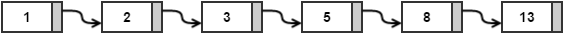
\includegraphics[width=\textwidth]{img/linkedList}
		\caption{\DIFaddFL{Liste chainée ordonnées}}
		\label{LinkedList}
	\end{figure}

	\DIFaddend \subsubsection*{Les alternatives}
	Il existe de nombreuses alternatives aux listes chainées pour trouver un élément plus rapidement: les tables de \DIFdelbegin \DIFdel{hashages }\textit{\DIFdel{(figure b)}}%DIFAUXCMD
\DIFdelend \DIFaddbegin \DIFadd{hashage }\cref{hashing}\DIFaddend , les arbres binaires \DIFdelbegin \textit{\DIFdel{(figure c)}}%DIFAUXCMD
\DIFdelend \DIFaddbegin \cref{tree}\DIFaddend , etc. Mais certaines séquences d'insertions peuvent être catastrophiques. Par exemple, insérer des éléments croissants dans un arbre binaire provoque un rééquilibrage de l'arbre. En revanche, si les éléments sont insérés de façon aléatoire, l'équilibrage devient plus rare.

	Grâce aux probabilités, les \og skip-list \fg{} \DIFdelbegin \textit{\DIFdel{(figure d)}} %DIFAUXCMD
\DIFdelend \DIFaddbegin \cref{skip} \DIFaddend bénéficient d'un atout majeur: aucune séquence ne peut provoquer systématiquement le pire scénario. Mieux encore, les skip-lists utilisent des algorithmes plus simples \DIFdelbegin \DIFdel{et rapides }\DIFdelend que ses concurrents.
	\DIFdelbegin \DIFdel{Les skip-lists sont aussi très légères et peuvent être configurées pour n'utiliser que $1\frac{1}{3}$ pointeur par élément.
	}\DIFdelend 

	\DIFdelbegin %DIFDELCMD < \begin{center}
%DIFDELCMD < 		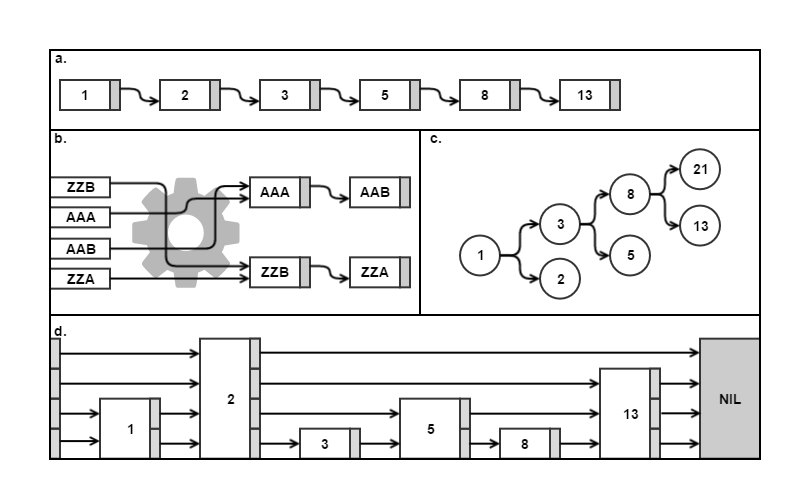
\includegraphics[width=\textwidth]{img/datastructure}
%DIFDELCMD < 	\end{center}
%DIFDELCMD < 	%%%
\DIFdelend \DIFaddbegin \begin{figure}[h]
		\centering
		\subfloat[Table de hashage] {
			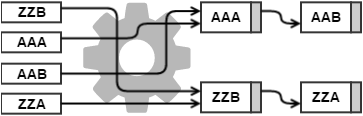
\includegraphics[scale=0.75]{img/hashing}
			\label{hashing}
		}
		\subfloat[Arbre binaire] {
			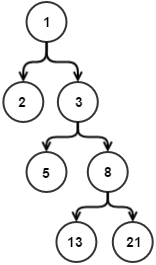
\includegraphics[scale=0.75]{img/tree}
			\label{tree}
		}
		\caption{\DIFaddFL{Différentes structures de données}}
	\end{figure}
	\begin{figure}
		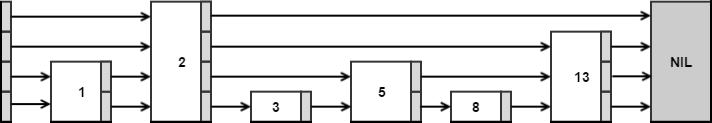
\includegraphics[width=\textwidth]{img/skip}
		\caption{\DIFaddFL{Skip-list}}
		\label{skip}
	\end{figure}
	\DIFaddend 

	\newpage
	\subsection{Skip-List}
	\DIFaddbegin 

	
	\DIFaddend Tout comme un dictionnaire, une skip-list permet de récupérer la définition d'un terme recherché \textit{(dit clé)}. Cette recherche est rapide, car les éléments \DIFaddbegin \textit{\DIFadd{(dit nœud)}} \DIFaddend présents dans un dictionnaire sont triés \DIFdelbegin \DIFdel{, et qu'}\DIFdelend \DIFaddbegin \DIFadd{et }\DIFaddend il est possible de commencer une exploration plus approfondie à un endroit précis.
	Une skip-list bénéficie des avantages de la liste chainée, en limitant fortement ses inconvénients. Cette structure de données utilise les chaines de façon parallèle. Une fonction basée sur des probabilités permet de déterminer \DIFdelbegin \DIFdel{si une nouvelle chainedoit figurer en parallèle ou non. Cette couche supérieure est un moyen plus rapide }\DIFdelend \DIFaddbegin \DIFadd{la hauteur de la chaine. Plus cette hauteur est élevée, moins la liste contient d'éléments. Une couche haute est donc un accès plus rapide vers des éléments plus loin dans la liste.
	}

	
	
	\DIFadd{Afin d'illustrer la skip-liste, il faut l'imaginer comme un réseau de transport en commun idéal où le temps d'attente des correspondances est nul. Un nœud dans la skip-liste est un arrêt obligatoire dans lequel un passager peut changer de moyen de locomotion. La couche la plus basse dans la skip-liste peut-être interprétée comme un bus. Il s'arrête à chacun de ses arrêts prévus, son temps de parcours est très lent. La couche n}\degree2\DIFadd{, plus rapide, est un métro. La couche n}\degree3\DIFadd{, un train. Si un passager souhaite aller voir un concert à Bruxelles alors qu'il est à la gare de Charleroi, il ne va pas faire le trajet en bus. Il est tout naturel et plus rapide dans ce cas de prendre dans un premier temps le train, puis le métro afin qu'il se rapproche le plus près possible du concert. Si le dernier arrêt de métro n'a pas permis }\DIFaddend d'accéder à \DIFdelbegin \DIFdel{cet élément.
	}\subsubsection*{\DIFdel{Définition}}
	%DIFAUXCMD
\DIFdelend \DIFaddbegin \DIFadd{la salle du concert, seulement dans ce cas le passager doit emprunter le bus.
	}\DIFaddend 

	\DIFdelbegin %DIFDELCMD < \begin{center}
%DIFDELCMD < 		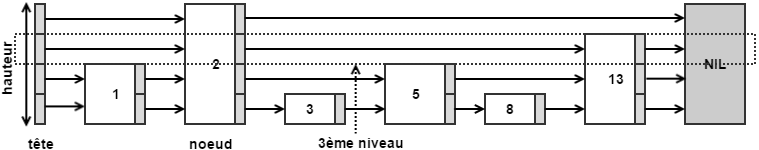
\includegraphics[width=\textwidth]{img/struct} %%%
%DIF < % TODO: Changer niveau par couche
	%DIFDELCMD < \end{center}
%DIFDELCMD < 	%%%
\DIFdelend \DIFaddbegin \begin{figure}[h!]
		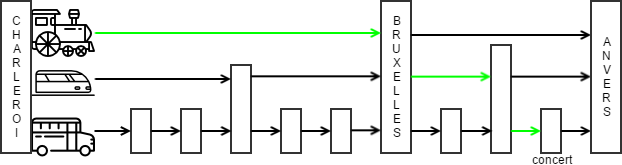
\includegraphics[width=\textwidth]{img/metaphore}
		\caption{\DIFaddFL{Métaphore d'une skip-liste par un réseau de transport en commun}}
		\label{skip-meta}
	\end{figure}
	\DIFaddend 

	\DIFdelbegin %DIFDELCMD < \begin{itemize}
%DIFDELCMD < 		\item %%%
\DIFdelend \DIFaddbegin \subsubsection*{\DIFadd{Définition}}
	\DIFaddend La hauteur maximale d'une skip-list est définie lors de sa création. Bien qu'il n'y ait pas de taille maximale d'une skip-list, il est conseillé d'utiliser $log_2(n)$ où $n$ est le nombre d'éléments théoriques présents dans la liste.
	\DIFdelbegin %DIFDELCMD < \item %%%
\DIFdel{Le niveau le plus bas de la liste mène }\DIFdelend \DIFaddbegin 

	\DIFadd{L'insertion dans la liste utilise une fonction basée sur la probabilité $p$ afin de définir sa hauteur maximale. Si $p$ vaut $\frac{1}{2}$, ça signifie que le nœud a une probabilité de $\frac{1}{2}$ d'être de hauteur 2, et a une probabilité $\frac{1}{4}$ d'être de hauteur 3. Un nœuds de hauteur $h$ possède $h$ pointeur. Un nœud de hauteur 3 a donc un accès }\DIFaddend au nœud suivant \DIFdelbegin \DIFdel{. %DIF < % TODO: Cette phrase est floue, à reformuler.
		}%DIFDELCMD < \item %%%
\DIFdel{Les }\DIFdelend \DIFaddbegin \DIFadd{de hauteur 3, ainsi que celui de hauteur 2 et 1.
	}

	\DIFadd{En raison des probabilités, les }\DIFaddend nœuds supérieurs \DIFdelbegin \DIFdel{pointent }\DIFdelend \DIFaddbegin \DIFadd{possèdent un pointeur }\DIFaddend vers un nœud plus avancé dans la liste. Une couche supérieure est \DIFdelbegin \DIFdel{une voie rapide vers la couche inférieure}\DIFdelend \DIFaddbegin \DIFadd{donc une voie plus rapide}\DIFaddend . Ainsi, la couche la plus haute contient les plus grands sauts\DIFdelbegin \DIFdel{.
		}%DIFDELCMD < \item %%%
\DIFdelend \DIFaddbegin \DIFadd{, et la couche la plus basse permet d'accéder à chacun des éléments.
		}

	\DIFaddend Le parcours d'une skip-list se fait de haut en bas, et de \DIFaddbegin \DIFadd{gauche à }\DIFaddend droite\DIFdelbegin \DIFdel{à gauche }\DIFdelend . Si la clé de l'élément suivant sur une couche est plus grande que celle qu'on recherche, celle-ci continue sur une voie inférieure.	
	\DIFdelbegin %DIFDELCMD < \item %%%
\DIFdel{L'insertion dans }\DIFdelend \DIFaddbegin 

	\begin{figure}[h]
		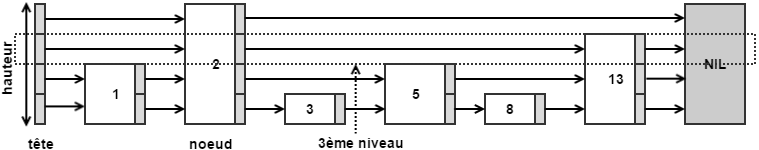
\includegraphics[width=\textwidth]{img/struct}
		\caption{\DIFaddFL{Structure d'une skip-list}}
		\label{StructSkip}
	\end{figure}

	\subsection{\DIFadd{La hauteur}}
	\DIFadd{La notion de hauteur est très importante dans une skip-liste. En effet, celle-ci permet de définir à combien de nœuds un élément est attaché. Si trop d'éléments possèdent la même hauteur, la recherche devient trop lente.	Cette méthode est définie à l'aide d'une fonction aléatoire. La hauteur ne dépend ni de }\DIFaddend la \DIFdelbegin \DIFdel{liste utilise une fonction }\DIFdelend \DIFaddbegin \DIFadd{clé de l'élément ni de sa valeur. La fonction aléatoire doit être définie pour qu'un élément de hauteur $h$ possède le double de probabilités qu'un élément de hauteur $h+1$. Ainsi, si un nœud de hauteur 1 a une probabilité $p$ }\DIFaddend de \DIFaddbegin \DIFadd{$0.5$ alors le niveau 2 a une }\DIFaddend probabilité \DIFdelbegin \DIFdel{afin de définir sa hauteur maximale.
		}%DIFDELCMD < \end{itemize}
%DIFDELCMD < 	%%%
\DIFdelend \DIFaddbegin \DIFadd{de $0.25$.
		}\DIFaddend 

	\newpage
	\section{Les algorithmes}
	Une skip-list a besoin d'avoir un pointeur vers sa tête $(node* head)$. La liste doit connaitre le nombre de \DIFdelbegin \DIFdel{voies actuellement utilisé $(size)$}\DIFdelend \DIFaddbegin \DIFadd{niveaux actuellement utilisés $(level)$}\DIFaddend . Selon les implémentations, il est possible de définir un nombre de \DIFdelbegin \DIFdel{voies }\DIFdelend \DIFaddbegin \DIFadd{couches }\DIFaddend maximal $(levelMAX)$. Il est aussi possible de changer le paramètre $(p)$ de probabilité de création d'une nouvelle \DIFdelbegin \DIFdel{voie}\DIFdelend \DIFaddbegin \DIFadd{couche}\DIFaddend . La variation de \DIFdelbegin \DIFdel{ses }\DIFdelend \DIFaddbegin \DIFadd{ces }\DIFaddend deux derniers paramètres est étudiée dans le chapitre \nameref{perf}.
	\DIFaddbegin \DIFadd{Un nœud contient une clé $key$ , une valeur $value$ ainsi qu'un tableau de pointeur vers les nœuds suivants $forward$. Il n'est pas nécessaire d'enregistrer la hauteur d'un nœud dans celui-ci.
	}\DIFaddend \lstinputlisting[linerange=BEGINSKStruct-ENDSKStruct]{SkipList/SkipList.h}

	L'initiation se fait de la manière suivante:
	\begin{itemize}
		\item La hauteur maximale est déterminée par le nombre d'éléments totaux $(n)$ \DIFdelbegin \DIFdel{présent }\DIFdelend \DIFaddbegin \DIFadd{présents }\DIFaddend dans la liste. Pour des questions de rapidité, la valeur $log_2(n)$ est recommandée.
		\item Création d'un élément $NIL$ possédant une clé plus grande que le maximum autorisé. \DIFaddbegin \DIFadd{Cette élément est aussi appelé }\textit{\DIFadd{élément bidon}}\DIFadd{.
		}\DIFaddend \item Définitions \DIFdelbegin \DIFdel{dès }\DIFdelend \DIFaddbegin \DIFadd{de }\DIFaddend ses pointeurs $forward$ vers lui-même.
		\item Le nombre de voies actuelles est fixé à 1.
		\item Le pointeur de tête est défini par cet élément $NIL$.
	\end{itemize}
	\emph{\DIFdelbegin \DIFdel{L}\DIFdelend \DIFaddbegin \DIFadd{La création d}\DIFaddend '\DIFdelbegin \DIFdel{algorithme écrit }\DIFdelend \DIFaddbegin \DIFadd{une skip-liste }\DIFaddend en langage C figure en annexe \ref{SKInit}.}

	\DIFaddbegin \begin{figure}[h]
		\DIFaddendFL 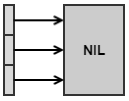
\includegraphics{img/init}
		\DIFaddbeginFL \caption{\DIFaddFL{Initialisation d'une skip-liste}}
		\label{SkipInit}
	\end{figure}
	\DIFaddend 

	\DIFaddbegin \newpage
	\DIFaddend \subsection{La recherche}
	\DIFaddbegin \DIFadd{De manière générale, pour rechercher dans une skip-list il suffit de commencer par le niveau le plus haut et d'effectuer une recherche élément par élément. Si l'élément suivant devient plus grand que celui recherché, il suffit alors de descendre d'un niveau dans la liste.
	}

	\DIFadd{Algorithmiquement parlant, }\DIFaddend La recherche d'un élément s'exécute de la façon suivante:
	\begin{enumerate}
		\item Commencer l'exploration de la liste par l'élément en tête, et se positionner sur la plus haute voie.
		\item Sur la voie actuelle, regarder la clé de l'élément suivant.
		\item \DIFdelbegin \DIFdel{S'}\DIFdelend \DIFaddbegin \DIFadd{Si }\DIFaddend elle est plus grande et qu'il existe une voie inférieure, descendre d'une voie.
		\item Sinon aller en 2.
		\item Si la clé de l'élément suivant correspond à celle qui est recherchée: l'élément a été trouvé.
		\item Sinon, l'élément n'a pas été trouvé.
	\end{enumerate}
	\DIFaddbegin 

	\DIFaddend \emph{L'algorithme écrit en langage C figure en annexe \ref{SKSearch}.}
	\DIFdelbegin %DIFDELCMD < \begin{center}
%DIFDELCMD < 		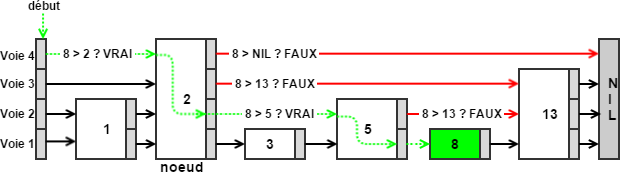
\includegraphics[width=\textwidth]{img/search}
%DIFDELCMD < 	\end{center}
%DIFDELCMD < 	%%%
\DIFdelend 

	\DIFdelbegin \subsection{\DIFdel{La hauteur}}
	%DIFAUXCMD
\addtocounter{subsection}{-1}%DIFAUXCMD
\DIFdel{La notion de hauteur est très importante dans une skip-liste.
		En effet, celle-ci permet de définir à combien de nœuds un élément est attaché. Si trop d'éléments possèdent la même hauteur}\DIFdelend \DIFaddbegin \subsubsection*{\DIFadd{Exemples}}	
	\paragraph*{\DIFadd{Comment rechercher l'élément 8 dans }\cref{SkipSearch1}\DIFadd{?}}
	\begin{itemize}
		\item \DIFadd{Se positionner sur la couche la plus haute: La 4ème voie.
		}\item \DIFadd{8 est-il plus grand que 2 ? Oui, se positionner sur le nœud 2.
		}\item \DIFadd{8 est-il plus grand que $+\infty$ }\textit{\DIFadd{(NIL)}}\DIFadd{? Non, descendre sur la 3ème voie.
		}\item \DIFadd{8 est-il plus grand que 13  ? Non, descendre sur la 2ème voie.
		}\item \DIFadd{8 est-il plus grand que 5 ? Oui, se positionner sur le nœud 5.
		}\item \DIFadd{8 est-il plus grand que 13 ? Non, descendre sur la 1ère voie.
		}\item \DIFadd{8 est-il plus grand que 8 ? Non, Il n'existe pas de voie plus basse.
		}\item \DIFadd{5 est le dernier nœud parcouru. L'élément suivant sur la voie 1 est 8. 8 est-il l'élément recherché? Oui}\DIFaddend , la recherche \DIFdelbegin \DIFdel{devient trop lente.
	Cette méthode est définie à l'aide }\DIFdelend \DIFaddbegin \DIFadd{est concluante.
	}\end{itemize}
	\begin{figure}[h]
		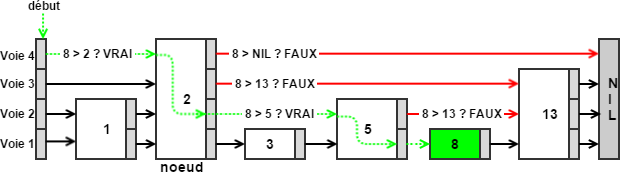
\includegraphics[width=\textwidth]{img/search}
		\caption{\DIFaddFL{Recherche de l'élément 8 dans une skip-liste}}
		\label{SkipSearch1}
	\end{figure}

	\newpage
	\paragraph*{\DIFadd{Comment rechercher l'élément 9 dans }\cref{SkipSearch2}\DIFadd{?}}

	\begin{itemize}
		\item \DIFadd{Se positionner sur la couche la plus haute: La 4ème voie.
		}\item \DIFadd{8 est-il plus grand que 2 ? Oui, se positionner sur le nœud 2.
		}\item \DIFadd{8 est-il plus grand que $+\infty$ }\textit{\DIFadd{(NIL)}}\DIFadd{? Non, descendre sur la 3ème voie.
		}\item \DIFadd{8 est-il plus grand que 13  ? Non, descendre sur la 2ème voie.
		}\item \DIFadd{8 est-il plus grand que 5 ? Oui, se positionner sur le nœud 5.
		}\item \DIFadd{8 est-il plus grand que 13 ? Non, descendre sur la 1ère voie.
		}\item \DIFadd{8 est-il plus grand que 8 ? Non, Il n'existe pas de voie plus basse.
		}\item \DIFadd{5 est le dernier nœud parcouru. L'élément suivant sur la voie 1 est 9. 9 est-il l'élément recherché? Non, la recherche est infructueuse.
	}\end{itemize}
	\begin{figure}[h]
		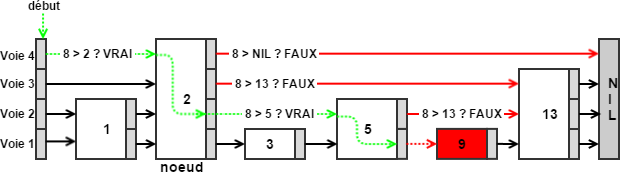
\includegraphics[width=\textwidth]{img/search2}
		\caption{\DIFaddFL{Recherche de l'élément 9 dans une skip-liste}}
		\label{SkipSearch2}
	\end{figure}

	
	\newpage
	\subsection{\DIFadd{L'insertion}}
	\DIFadd{L'insertion }\DIFaddend d'une \DIFdelbegin \DIFdel{fonction aléatoire. La hauteur ne dépend ni de la clé de l'élément ni de sa valeur. La fonction aléatoire doit être définie pour }\DIFdelend \DIFaddbegin \DIFadd{entrée dans une skip-list est essentiellement la même chose que la recherche. A l'exception }\DIFaddend qu'un \DIFdelbegin \DIFdel{élément de hauteur $h$ possède le double de probabilité qu'un élément de hauteur $h+1$. Ainsi, si un nœud de hauteur 1 a une probabilité $p$ de $0.5$ alors le niveau2 a une probabilité de $0.25$}\DIFdelend \DIFaddbegin \DIFadd{tableau $update$, de taille identique à la hauteur de la liste, est utilisé pour mémoriser les pointeurs de chaque élément avant de descendre d'un niveau. Ce tableau est utilisé pour mettre à jour les liens nécessaires pour que la structure de donnée reste cohérente}\DIFaddend .

	\DIFdelbegin \subsection{\DIFdel{L'insertion}}
	%DIFAUXCMD
\addtocounter{subsection}{-1}%DIFAUXCMD
\DIFdel{L}\DIFdelend \DIFaddbegin \DIFadd{Algorithmiquement parlant, l}\DIFaddend 'insertion d'un élément dans une skip-liste s'effectue de la façon suivante:
	\begin{enumerate}
		\item Commencer l'exploration de la liste par l'élément en tête, et se positionner sur la plus haute voie.
		\item Sur la voie actuelle, regarder la clé de l'élément suivant.
		\item Si elle est plus grande et qu'il existe une voie inférieure, marquer ce \DIFdelbegin \DIFdel{nœud}\DIFdelend \DIFaddbegin \DIFadd{pointeur}\DIFaddend . Puis, descendre d'une voie.
		\item Sinon aller en 2.
		\item Si la clé de l'élément suivant correspond à celle qui est recherchée: modifier la valeur de l'élément par celle de la valeur à insérer. \textbf{FIN}.
		\item Sinon, appeler la fonction de probabilité pour récupérer sa valeur $n$.
		\item Si $n$ est plus grand que la hauteur $h$ de la liste, mettre à jour les pointeurs supérieurs à $h$ vers $NIL$. Ensuite, définir la hauteur maximum actuelle $h$ à $n$.
		\item Créer le nœud $x$ de hauteur $n$.
		\item Pour chaque voie de $1$ à $n$.
		\item Mettre à jour les pointeurs de $x$ vers l'élément suivant de l'élément marqué de cette voie.
		\item Mettre à jour les pointeurs de l'élément marqué de cette voie vers $x$.
		\item \textbf{FIN}.
	\end{enumerate}
	\emph{L'algorithme écrit en langage C est présenté en annexe \ref{SKInsert}.}
	\DIFdelbegin %DIFDELCMD < \begin{center}
%DIFDELCMD < 		%%%
\DIFdelend \DIFaddbegin 

	\newpage
	\subsubsection*{\DIFadd{Exemples}}	
	\paragraph*{\DIFadd{Comment insérer l'élément 8 dans }\cref{SkipInsert1}\DIFadd{?}}
	\begin{itemize}
		\item \DIFadd{Se positionner sur la couche la plus haute: La 4ème voie.
		}\item \DIFadd{8 est-il plus grand que 2 ? Oui, se positionner sur le nœud 2.
		}\item \DIFadd{8 est-il plus grand que $+\infty$ }\textit{\DIFadd{(NIL)}}\DIFadd{? Enregistrer ce lien en mémoire, puis descendre sur la 3ème voie.
		}\item \DIFadd{8 est-il plus grand que 13  ? Enregistrer ce lien en mémoire, puis descendre sur la 2ème voie.
		}\item \DIFadd{8 est-il plus grand que 5 ? Oui, se positionner sur le nœud 5.
		}\item \DIFadd{8 est-il plus grand que 13 ? Enregistrer ce lien en mémoire, puis descendre sur la 1ère voie.
		}\item \DIFadd{8 est-il plus grand que 8 ? Enregistrer ce lien en mémoire, Il n'existe pas de voie plus basse.
		}\item \DIFadd{5 est le dernier nœud parcouru. L'élément suivant sur la voie 1 est 8. 8 est-il l'élément recherché? Non, on crée un nouvel élément. Générer une hauteur aléatoire: hauteur 1.
		}\item \DIFadd{Ajouter un lien du nouvel élément 8 en voie 1. Ce lien doit pointer vers l'élément du lien enregistré à cette même voie. Il s'agit de l'élément 13.
		}\item \DIFadd{Modifier ce lien enregistré en voie 1 (de l'élément 5 vers l'élément 13) pour qu'il pointe vers ce nouvel élément 8.
		}\item \DIFadd{FIN.
	}\end{itemize}
	\begin{figure}[h]
		\DIFaddendFL 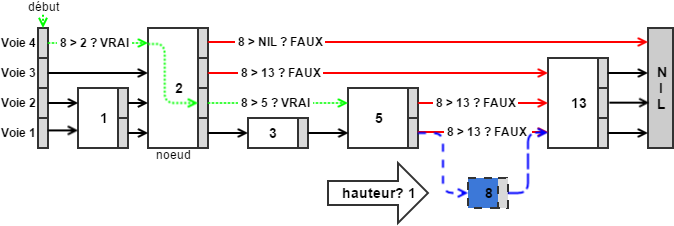
\includegraphics[width=\textwidth]{img/insert}
		\DIFdelbeginFL %DIFDELCMD < \end{center}
%DIFDELCMD < 	%%%
\DIFdelendFL \DIFaddbeginFL \caption{\DIFaddFL{Insertion dans une skip-liste}}
		\label{SkipInsert1}
	\end{figure}
	\DIFaddend 

	\DIFaddbegin \newpage
	\paragraph*{\DIFadd{Comment insérer l'élément 5 dans }\cref{SkipInsert1}\DIFadd{?}}
	\begin{itemize}
		\item \DIFadd{Se positionner sur la couche la plus haute: La 4ème voie.
		}\item \DIFadd{5 est-il plus grand que 2 ? Oui, se positionner sur le nœud 2.
		}\item \DIFadd{5 est-il plus grand que $+\infty$ }\textit{\DIFadd{(NIL)}}\DIFadd{? Enregistrer ce lien en mémoire, puis descendre sur la 3ème voie.
		}\item \DIFadd{5 est-il plus grand que 13 ? Enregistrer ce lien en mémoire, puis descendre sur la 2ème voie.
		}\item \DIFadd{5 est-il plus grand que 13 ? Enregistrer ce lien en mémoire, puis descendre sur la 1ère voie.
		}\item \DIFadd{5 est-il plus grand que 3 ? Oui, se positionner sur le nœud 3.
		}\item \DIFadd{5 est-il plus grand que 8 ? Enregistrer ce lien en mémoire, Il n'existe a pas de voie plus basse.
		}\item \DIFadd{5 est le dernier nœud parcouru. L'élément suivant sur la voie 1 est 8. 8 est-il l'élément recherché? Non, on crée un nouvel élément. Générer une hauteur aléatoire: hauteur 2.
		}\item \DIFadd{Ajouter un lien du nouvel élément 5 en voie 1. Ce lien doit pointer vers l'élément du lien enregistré à cette même voie. Il s'agit de l'élément 8.
		}\item \DIFadd{Modifier ce lien enregistré en voie 1 (de l'élément 3 vers l'élément 8) pour qu'il pointe vers ce nouvel élément 5.
		}\item \DIFadd{Ajouter un lien du nouvel élément 5 en voie 2. Ce lien doit pointer vers l'élément du lien enregistré à cette même voie. Il s'agit de l'élément 13.
		}\item \DIFadd{Modifier ce lien enregistré en voie 2 (de l'élément 2 vers l'élément 13) pour qu'il pointe vers ce nouvel élément 5.
		}\item \DIFadd{FIN.
	}\end{itemize}
	\begin{figure}[h]
		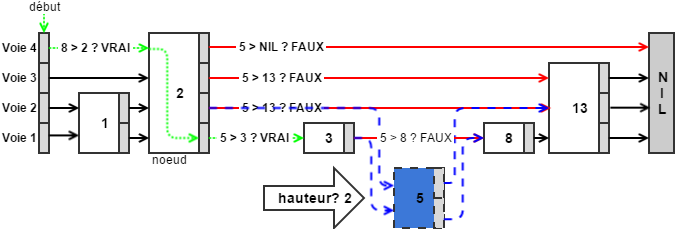
\includegraphics[width=\textwidth]{img/insert2}
		\caption{\DIFaddFL{Insertion dans une skip-liste}}
		\label{SkipInsert2}
	\end{figure}

	\newpage
	\DIFaddend \subsection{La suppression}
	La suppression d'un élément dans une skip-liste s'effectue de la façon suivante:
	\begin{enumerate}
		\item Commencer l'exploration de la liste par l'élément en tête, et se positionner sur la plus haute voie.
		\item Sur la voie actuelle, regarder la clé de l'élément suivant.
		\item Si elle est plus grande et qu'il existe une voie inférieure, marquer ce nœud. Puis, descendre d'une voie.
		\item Sinon aller en 2.
		\item Si la clé de l'élément suivant ne correspond pas à celle qui est recherchée, \textbf{FIN}.
		\item Sinon pour chaque niveau de l'élément trouvé $x$, mettre à jour les pointeurs de l'élément marqué de cette voie vers l'élément suivant de $x$.
		\item Supprimer $x$.
		\item Si l'élément de tête de la hauteur actuelle de la liste pointe vers $NIL$, diminuer la hauteur actuelle de la liste de 1.
		\item Sinon, \textbf{FIN}.
		\item Si la hauteur est plus grande que 1, aller en 8.
	\end{enumerate}
	\emph{L'algorithme écrit en langage C figure en annexe \ref{SKDelete}.}
	\begin{center}
		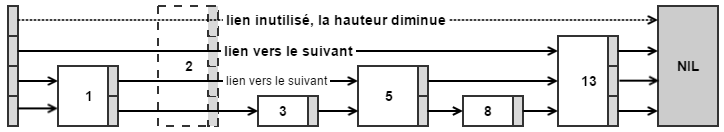
\includegraphics[width=\textwidth]{img/delete}
	\end{center}

	\DIFaddbegin \newpage
	\DIFaddend \section{Analyse des performances}\label{perf}
	\DIFaddbegin \DIFadd{La caractéristique majeure de la skip-list est l'aléatoire. L'insertion d'un élément nouveau utilise une hauteur qui est déterminée par le hasard. De ce fait, une même séquence produira une liste différente. Cela a comme conséquence qu'aucune séquence prédéterminée de nombres ne peut produire une dégradation des performances, contrairement aux arbres binaires qui eux doivent être constamment rééquilibrés.
	}

	\DIFadd{De par sa nature probabiliste, on suppose que l'utilisateur n'aura pas un comportement à vouloir dégénérer volontairement la liste. C'est-à-dire que les performances peuvent être dégradées en retirant consciemment les éléments après avoir inspecté leur hauteur. Si l'utilisateur supprime tous les nœuds de hauteur $h>1$, le pire scénario de la skip-list équivaut à une liste chainée classique.
	}

	\DIFadd{Le temps requis pour exécuter l'insertion et la suppression dans une skip-list est prédominé par le temps de la recherche d'un élément. Ces deux derniers n'ont qu'un cout supplémentaire constant par rapport à la hauteur de la liste; alors que le cout de la recherche est proportionnel à la longueur du chemin à parcourir.
	}

	
	\subsection{\DIFadd{Analyse pour $p=\frac{1}{2}$}}
	\DIFadd{Pour une variable aléatoire $p=\frac{1}{2}$ et une skip-list de taille infinie, celle-ci tend à ce que chacun des niveaux possèdent $\frac{1}{2}$ moins d'éléments. Ainsi, le niveau 1 contient $n$ élément, le niveau 2 $\frac{n}{2}$, le niveau 3 $\frac{n}{4}$, ..., un élément à hauteur $h$: $\frac{n}{{2}^{h-1}}$. Par conséquent, le nombre total de liens dans une skip-list équivaut à }\[\DIFadd{n+\frac{n}{2}+\frac{n}{4}+\frac{n}{8}+\dots = \sum_{h=1}^{+\infty}\frac{n}{{2}^{h-1}}=2n}\] \DIFadd{Ce qui signifie qu'en moyenne un élément dans une skip-list possède 2 liens. Vu que la recherche se fait de haut en bas et de gauche à droite, chaque clé examinée à un niveau précis ($i$) ne peut pas appartenir à un niveau supérieur ($i+1$).
	De ce fait, on peut déduire qu'en moyenne le nombre de fois que l'on avance dans la liste à un niveau précis équivaut au nombre de liens divisé par le nombre d'éléments, soit $\frac{2n}{n}=2$.
	}

	\newpage
	\DIFadd{La probabilité qu'un élément soit de hauteur $i$ est de ${p^{i}} = \frac{1}{2^{i}} $. Le facteur $p$ est constant ($\frac{1}{2}$), la probabilité de la hauteur des clés est équiprobable. Si l'on additionne la probabilité de hauteur chacune des clés de la skip-list, et que l'on prend $h$ comme hauteur de la liste, on déduit la formule suivante.
	}\[\DIFadd{
		\frac{1}{{2}^{1}}+\frac{1}{{2}^{2}}+\frac{1}{{2}^{3}}+\dots+\frac{1}{{2}^{h}}
		= \sum _{i=1}^{h} (}{\DIFadd{\frac{1}{2}}}\DIFadd{)^{i}
	}\]
	\DIFadd{Cette hauteur, il est possible de l'estimer. Si $h$ tend vers l'infini, la série converge vers 1. Ce qui a comme conséquence:
	}\[\DIFadd{
		n}{\DIFadd{(\frac{1}{2})}}\DIFadd{^{h} = 1
		\iff }{\DIFadd{(\frac{1}{2})}}\DIFadd{^{h}=\frac{1}{n}
		\iff h = \log_{\frac{1}{2}}(\frac{1}{n})
		\iff h = \log_{2}(n)
	}\]

	\DIFadd{L'algorithme de recherche effectue possède 2 boucles imbriquées. La boucle la plus profonde permet d'avancer de gauche à droite dans la liste. Pour $p=\frac{1}{2}$, en moyenne celle-ci avance de $2$. La boucle supérieure quant à elle varie selon la hauteur de la liste. La hauteur est estimée, avec une forte probabilité, à $\log_{2} n $. Si l'on combine les 2 estimations, nous avons donc une forte probabilité que la recherche s'effectue en $\log_{2}( 2n )$ opérations, soit $\mathcal{O}(log(n))$.
	}

	
	\subsection{\DIFadd{Généralisation}}

	\DIFadd{Le raisonnement utilisé précédemment pour $p=\frac{1}{2}$ reste valable quelle que soit la valeur de $p$, voir }\cref{recap}\DIFadd{. Le raisonnement qui effectue une sommation servant au calcul de lien dans une liste convergera vers $\frac{n}{p}$. Par contre, la somme des probabilités ($p^1 + p^2 + p^3 + ... + p^k$), converge toujours vers $\frac{p}{1-p}$. 
	 	}

	 \begin{table}[h]
	 \begin{tabular}{|l|c|c|}
	 	\hline
	 	\DIFaddFL{Scénario }& \DIFaddFL{attendu }& \DIFaddFL{pire }\\
	 	\hline
	 	\DIFaddFL{Nombre d'élément }& \DIFaddFL{$n$ }& \DIFaddFL{$n$ }\\ 
	 	\hline
	 	\DIFaddFL{Hauteur }& \DIFaddFL{$log_{\frac{1}{p}} n$ }& \DIFaddFL{$\infty$ }\\ 
	 	\hline
	 	\DIFaddFL{Nombre de lien }& \DIFaddFL{$n/p$ }& \DIFaddFL{$n*h$ }\\ 
	 	\hline
	 	\DIFaddFL{Recherche }& \DIFaddFL{$\mathcal{O}(\log n)$ }& \DIFaddFL{$\mathcal{O}(n)$ }\\ 
	 	\hline
	 	\DIFaddFL{Insertion }& \DIFaddFL{$\mathcal{O}(\log n)$ }& \DIFaddFL{$\mathcal{O}(n)$ }\\
	 	\hline
	 	\DIFaddFL{Suppression }& \DIFaddFL{$\mathcal{O}(\log n)$ }& \DIFaddFL{$\mathcal{O}(n)$}\\
	 	\hline
	 \end{tabular}
	 \caption{\DIFaddFL{Tableau récapitulatif}}
	 \label{recap}
	 \end{table}

	 \subsubsection*{\DIFadd{Le pire cas}}

	 \DIFadd{Les ordinateurs ne possèdent pas une mémoire infinie. Par conséquent, il est impossible d'ajouter une infinité d'éléments. C'est pourquoi à la création d'une skip-list, la hauteur maximale est bornée par la formule du cas attendu avec une forte probabilité. Le pire scénario de hauteur infinie est donc impossible. Dans le cas très improbable que chacun des éléments de la skip-list soit à cette hauteur maximale, nous avons une recherche en $n*h$: soit $\mathcal{O}(n)$. 
	 	}

	 \DIFadd{De façon générale, avec une constance $c>1$ $h$ est plus grande que $c log n$ avec une probabilité d'au plus $\frac{1}{n^{c-1}}$. En d'autres mots, la probabilité que $h$ soit plus petit que $c log n$ est d'au moins $1-\frac{1}{n^{c-1}}$. Par conséquent, avec une forte probabilité, la hauteur d'une skip-liste est bien d'ordre $\mathcal{O}(log n)$. Par exemple: si $n=1000$, la probabilité est d'une sur un million.
	}

	
	\subsection{\DIFadd{Expérimentation}}

	\DIFadd{Les expérimentations suivantes ont été réalisées sur un ordinateur Windows 10 64 bits possédant un AMD FX 8350 et 16Gb de RAM. Les tests ont été lancés $10^5$ fois, les résultats présentés sont la moyenne de tous les tests. Les très légères différences avec les résultats attendu peuvent s'expliquer par la façon dont un ordinateur génère des nombres aléatoires. On parle d'ailleurs de nombre "pseudo" aléatoire.
	}

	\DIFadd{L'algorithme utilisé pour générer les nombres aléatoires dans ces tests est }\textit{\DIFadd{xoroshiro128+}}\DIFadd{. Il a été développé par David Blackman et Sebastiano Vigna. Il s'agit de l'algorithme le plus rapide aujourd'hui. Il est intéressant d'utiliser un générateur rapide afin de déterminer la hauteur d'un élément de la skip-list. L'utilisation de la fonction }\textit{\DIFadd{rand}} \DIFadd{de }\textit{\DIFadd{stdlib}} \DIFadd{permet d'insérer $10^7$ éléments en $5.792$ secondes, alors que l'algorithme }\textit{\DIFadd{xoroshiro128+}} \DIFadd{permet d'en insérer autant en $4.014$ secondes. Cette différence de $30\%$ n'est pas négligeable.
	}

	\begin{table}[h]
		\resizebox{\columnwidth}{!}{
			\begin{tabular}{|c|r|r|r|r|r|r|r|r|r|r|}
				\hline
				\backslashbox{p}{h} & 1 & 2 & 3 & 4 & 5 & 6 & 7 & 8 & 9 & 10 \\
				\hline
				4/5 & 1000.00 & 800.05 & 640.02 & 512.01 & 409.64 & 327.74 & 262.16 & 209.74 & 167.81 & 134.23 \\
				3/4 & 1000.00 & 749.97 & 562.52 & 421.83 & 316.34 & 237.25 & 177.98 & 133.45 & 100.10 & 75.07 \\
				2/3 & 1000.00 & 666.76 & 444.52 & 296.35 & 197.60 & 131.70 & 87.79 & 58.49 & 38.98 & 25.99  \\
				3/5 & 1000.00 & 600.00 & 360.00 & 216.02 & 129.61 & 77.77 & 46.66 & 28.00 & 16.79 & 10.06 \\
				1/2 & 1000.00 & 500.01 & 250.06 & 125.04 & 62.56 & 31.27 & 15.63 & 7.82 & 3.91 & 1.96 \\
				2/5 & 1000.00 & 399.96 & 160.02 & 64.01 & 25.60 & 10.23 & 4.09 & 1.63 & 0.00 & 0.00 \\
				1/3 & 1000.00 & 333.33 & 111.14 & 37.03 & 12.34 & 4.11 & 0.00 & 0.00 & 0.00 & 0.00 \\
				1/4 & 1000.00 & 249.97 & 62.48 & 15.63 & 3.90 & 0.00 & 0.00 & 0.00 & 0.00 & 0.00 \\
				1/5 & 1000.00 & 200.04 & 40.00 & 8.01 & 0.00 & 0.00 & 0.00 & 0.00 & 0.00 & 0.00 \\
				1/10 & 1000.00 & 100.01 & 10.02 & 0.00 & 0.00 & 0.00 & 0.00 & 0.00 & 0.00 & 0.00 \\
				1/20 & 1000.00 & 50.00 & 0.00 & 0.00 & 0.00 & 0.00 & 0.00 & 0.00 & 0.00 & 0.00 \\
				\hline
			\end{tabular}
		}
		\caption{\DIFaddFL{Le nombre d'éléments par niveau en fonction de $p$}}
		\label{tbRes1}
	\end{table}

	\subsubsection*{\DIFadd{Variation de p}}

	\DIFadd{Afin de vérifier que le $p$ à bien l'effet voulu, il suffit de compter le nombre d'éléments existants à chaque niveau. S'il y a $n$ éléments à la hauteur 1, on s'attend à obtenir $np$ éléments de hauteur 2 avec une forte probabilité.
	}

	\DIFadd{Dans les faits, en essayant différentes valeurs pour une skip-list de 1000 éléments, on  peut obtenir les résultats présents dans la }\cref{tbRes1}\DIFadd{. Le résultat obtenu, correspond à notre espérance: $p$ influence correctement la hauteur de la liste et par conséquent son poids. 
	}

	\DIFadd{Une question plus intéressante à se poser serait: Quel est la meilleure valeur pour $p$ ? Choisir un petit nombre réduit le nombre de liens dans la liste. Cela a comme conséquence de pouvoir faire de plus grand saut, mais moins souvent. Par exemple avec $p=0.1$, il sera fort probable de faire des sauts d'une dizaine d'éléments. Mais la recherche du 9ème élément se fera sur la couche la plus basse qui elle, est 10 fois lente. En revanche, choisir un grand nombre pour $p$, augmentera fortement le nombre de liens dans la skip-list. Celle-ci possède donc un grand nombre de hauteurs, et donc plus de saut. Cela a comme conséquence de faire plus souvent des sauts, mais ils seront plus petits.
	 }

	\begin{figure}[h]
		\centering
		\resizebox{0.8\columnwidth}{!}{
			\begin{tikzpicture}
			\begin{axis}[
				ymin=300,xmin=0.05,xmax=0.80,xtick distance=0.1,ytick distance=100,
				ylabel={Temps},
				xlabel=Valeur de $p$
			]
			\addplot+[smooth,mark min] table [x=p,y=1000] {data/pvar.dat};
			\addplot+[smooth,mark min] table [x=p,y=10000] {data/pvar.dat};
			\addplot+[smooth,mark min] table [x=p,y=100000] {data/pvar.dat};
			\addplot+[smooth,mark min] table [x=p,y=1000000] {data/pvar.dat};		
			\end{axis}
			\end{tikzpicture}
		}
		\caption{\DIFaddFL{Vitesse d'exécution en fonction de $p$}}
		\label{tbRes2}
	\end{figure}

	\DIFaddend \section{\DIFdelbegin \DIFdel{Comparaison }\DIFdelend \DIFaddbegin \DIFadd{Comparaisons }\DIFaddend avec d'autres structures\DIFdelbegin \DIFdel{de données}\DIFdelend }
	\DIFaddbegin \newpage
	\DIFaddend 

	
	\DIFdelbegin %DIFDELCMD < \begin{appendices}
%DIFDELCMD < 	%%%
\DIFdelend \newpage
	\DIFaddbegin \DIFadd{c
	}\newpage
	\DIFadd{d
	}\newpage

	\begin{appendices}
	\DIFaddend \section{Représentation d'une Skip-List en langage C}
	\subsection{Initiation}\label{SKInit}
	\lstinputlisting[linerange=BEGINSKInit-ENDSKInit]{SkipList/SkipList.c}
	\subsection{Fonction aléatoire}\label{SKRandom}
	\lstinputlisting[linerange=BEGINSKRandom-ENDSKRandom]{SkipList/SkipList.c}

	\subsection{Recherche}\label{SKSearch}
	\lstinputlisting[linerange=BEGINSKSearch-ENDSKSearch]{SkipList/SkipList.c}

	\subsection{Insertion}\label{SKInsert}
	\lstinputlisting[linerange=BEGINSKInsert-ENDSKInsert]{SkipList/SkipList.c}

	\subsection{Suppression}\label{SKDelete}
	\lstinputlisting[linerange=BEGINSKDelete-ENDSKDelete]{SkipList/SkipList.c}
	\newpage
	\end{appendices}

	
	@online{1,
		author = {Patrice Roy},
		title = {Skip Lists},
		date = {27/02/2016},
		url = {http://h-deb.clg.qc.ca/Sujets/Structures-donnees/SkipLists.html},
	}
	@online{2,
		author = {Sylvie Hamel},
		title = {Dictionnaires ordonnés et “Skip List”},
		date = {25/02/2016},
		url = {http://www.iro.umontreal.ca/~hamelsyl/SkipList.pdf},
	}

\end{document} 